%QUESTÃO - Cód.: TF1p0q01

\question [\questaopt] Um automóvel aproxima-se de um paredão, como ilustra a figura.

\begin{center}
	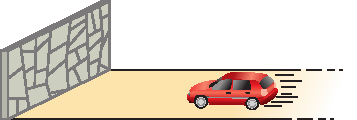
\includegraphics[width=0.7\linewidth]{questoes/imagens/TF1p02q10}
\end{center}


	\begin{EnvUplevel}
		
		\begin{choices}
	
			\choice o automóvel está em movimento em relação ao paredão.
			
			\choice o paredão está em movimento em relação ao automóvel.
			
			\choice o paredão está em repouso em relação ao solo.
			
			\choice o paredão está em repouso em relação ao automóvel.
			
			\correctchoice	o motorista está em repouso em relação ao automóvel, mas em	movimento em relação à superfície da Terra.
	
		
		\end{choices}
	\end{EnvUplevel}

%--------------------------SOLUÇÃO---------------------------------------

	\begin{solution}
		
Alternativa: {\bf E)} o motorista está em repouso em relação ao automóvel, mas em	movimento em relação à superfície da Terra.
		
	\end{solution}

